\chapter{Nachhaltigkeits Rosette}
\label{chap:rosette}

Für beide Systeme wird nun eine Nachhaltigkeitsrosette erstellt. Dabei besteht die Rosette aus drei Kategorien mit je vier Kriterien. Die Kategorien setzen sich zusammen aus Umwelt, Wirtschaft und Gesellschaft. Die Einteilung der Kriterien ist subjektiv, genauso wie die Bewertung der einzelnen.



\section{Bewertung}

\begin{figure}[h]
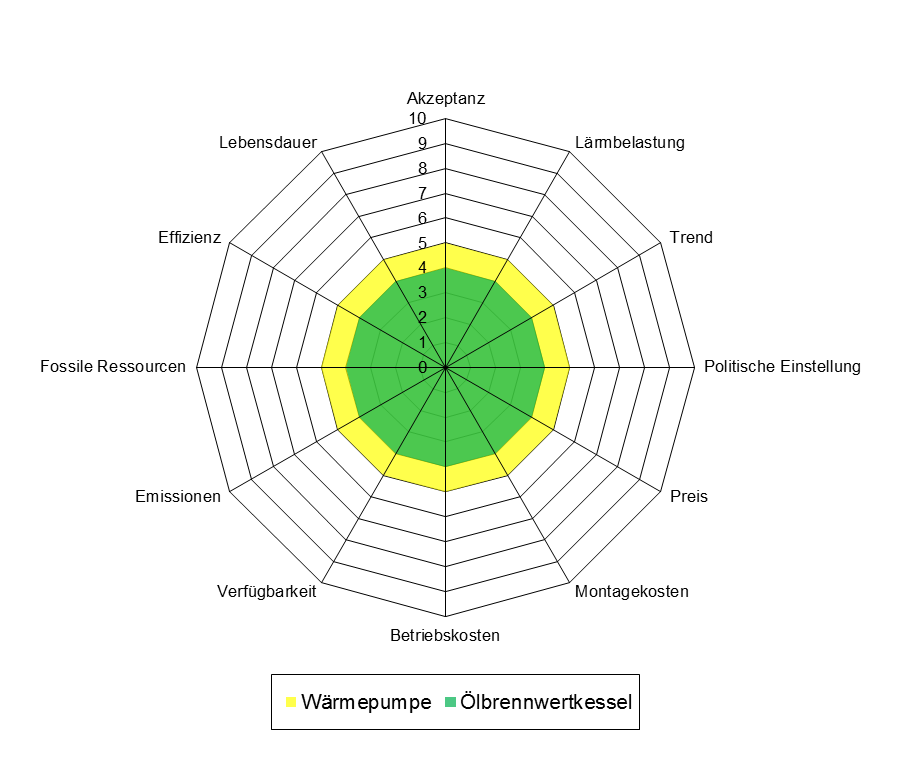
\includegraphics[scale=0.54]{bilder/Rosette.png}
\caption{Nachhaltigkeitsrosette}
\end{figure}

\begin{table}
\begin{center}
\begin{tabular}[c]{|p{0.25 \textwidth}|p{0.25 \textwidth}|p{0.25 \textwidth}|}

  \hline
  \textbf{Kriterium} &
  \textbf{Wärmepumpe} &
  \textbf{Ölbrennwertkessel} \\ \hline

  \multicolumn{3}{|c|}{\textbf{Umwelt}} \\ \hline
  
  Emissionen
  & 9 & 2 \\
  Fossile Ressourcen
  & 7 & 1 \\
  Effizienz
  & 8 & 7 \\
  Lebensdauer
  & 5 & 8 \\
  \hline
  
  \multicolumn{3}{|c|}{\textbf{Wirtschaft}} \\ \hline
  
  Preis
  & 4 & 8 \\
  Montagekosten
  & 4 & 7 \\
  Betriebskosten
  & 8 & 5 \\
  Verfügbarkeit
  & 5 & 8 \\
  \hline

  \multicolumn{3}{|c|}{\textbf{Gesellschaft}} \\ \hline

  Akzeptanz
  & 8 & 3 \\
  Lärmbelastung
  & 5 & 5 \\
  Trend
  & 7 & 4 \\
  Politische Einstellung
  & 7 & 3 \\
  \hline

\end{tabular}
\end{center}
\label{rosette:score}
\caption{Punktetabelle für die Nachhaltigkeitsrosette}
\end{table}


\subsection{Erklärungen}

\begin{itemize}

\item \textbf{Emissionen}: Wärmepumpe klar im Vorteil, da so gut wie keine Emissionen. Keine Maximalwertung da bei der Stromerzeugung Emissionen entstehen können.

\item \textbf{Fossile Ressourcen}: Wärmepumpe klar vorne, da die Ölheizung von ihrem Funktionsprinzip her vollständig auf fossile Ressourcen angewiesen ist.

\item \textbf{Effizienz}: Beide ziemlich ähnlich. Ölheizungen erreichen einen Wirkungsgrad von bis zu 97\%. Die Wärmepumpe braucht viel Strom, kann aber einen Grossteil der Wärme aus dem Erdkreislauf bekommen.

\item \textbf{Lebensdauer}: Wärmepumpen haben eine Lebensdauer von 15-20 Jahren \cite{fws:faq}. Bei den Ölbrennwertkesseln rechnet man mit 20-25 Jahren\cite{offerten24:oel}.

\item \textbf{Preis}: Für eine Ölheizung muss mit etwa 15'000 CHF{offerten24:oel} gerechnet werden. Bei einer Wärmepumpe betragen die Installationskosten etwa 35'000 CHF.{offerten24:wp}

\item \textbf{Montagekosten}: Ölheizung im Vorteil, da die Wärmepumpe aufwändige Bohrungen benötigt.

\item \textbf{Betriebskosten}: Wärmepumpe hat den Vorteil des Erdwärmekreislaufs. Dadurch muss nicht die ganze Wärmeleistung von aussen zugeführt werden, wie bei der Ölheizung.

\item \textbf{Verfügbarkeit}: Ölheizung benötigt nur ein Tank, welcher fast überall platziert werden kann. Die Wärmepumpe kann nicht überall eingesetzt werden, da tiefe Bohrungen notwendig sind, welche am Standort bewilligt werden müssen. 

\item \textbf{Akzeptanz}: Durch die Globalisierung wird die Nachhaltigkeit immer mehr betont. Dadurch ist die Akzeptanz für Wärmepumpen sicher um einiges höher, da Öl schnell mit Umweltverschmutzung in Verbindung gebracht wird.

\item \textbf{Lärmbelastung}: Die Solewasser-Wärmepumpe ist etwa gleich laut wie eine Ölheizung.

\item \textbf{Trend}: Ähnlich wie bei der Akzeptanz, begünstigen die Medien und die aktuelle Ressourcenlage den Trend nach nachhaltigeren Produkten und Systemen.

\item \textbf{Politische Einstellung}: Durch die Debatte des Atomausstiegs, wurde auch die Politik auf das Thema der Nachhaltigkeit aufmerksam. Dadurch sind Wärmepumpen sicher im Vorteil.

\end{itemize}
